\newpage
%
% Začiatok analýzy
% Úvod do analýzy
%
\ifthenelse {\boolean{bachelor}}
{
	%\section{Analysis}
	\section{Analýza} 
}
{
	%\chapter{Analysis}
	\chapter{Analyza}
}
V tejto kapitole priblížím a rozoberiem čo je spracovanie prirodzeného jazyka, jeho využitie v aplikáciach a systémoch a jeho hlavné úlohy. Ďalej zanalyzujem nástroje, ktoré sa dajú využiť na spracovanie prirodzeného jazyka a tak isto sa pozriem na aplikácie a systémy, ktorých základom je spracovanie textu.

%
% Spracovanie prirodzeného jazyka
%
\ifthenelse {\boolean{bachelor}}
{
	%\subsection{Subsection}
	\subsection{Spracovanie prirodzeného jazyka}
}
{
	%\section{Subsection}
	\section{Spracovanie prirodzeného jazyka}
}
\label{subsec:nlp}
Spracovanie prirodzeného jazyka (angl. Natural Language Processing - NLP) môže byť definované ako automatické alebo poloautomatické spracovanie ľudského jazyka~\cite{Copestake2004}. Počítače doposiaľ nedokážu plne porozumieť ľudskému jazyku, či už sa jedná o písaný alebo hovorový, a preto hlavným cieľom NLP je vybudovať výpočtové modely prirodzeného jazyka pre jeho analýzu a generovanie~\cite{Bharati1995}.

Porozumenie ľudskej reči je mnohokrát náročne aj pre samotných ľudí a nie to ešte pre počítače. Na svete je veľké množstvo jazykov, ktoré sa od seba líšia charakteristikami typickými pre konkrétny jazyk. Navyše, každý človek je odlišný a typický, čo spôsobuje, že výslovnosť rovnakého slova viacerými ľuďmi môže byť odlišná. Ďalej máme slangové slová a slová typické len pre určité územie. Pri spracovávaní prirodzeného jazyka treba vziať do úvahy tieto, a aj ďalšie, premenné. Dosiahnutie tohto cieľa je preto často veľmi náročné.

V súčastnosti najpoužívanejšie algoritmy na NLP využívajú strojové učenie. Dosiahnutie úplného porozumenia a spracovania ľudského prirodzeného jazyka by znamenalo vyriešiť \textit{AI-complete} problém, čo znamená, že obtiažnosť tohto problému je ekvivalentná s obtiažnosťou problému vytvorenia počítača inteligentného ako človek, takzvané ,,true AI''.

%
% Využitie spracovania prirodzeného jazyka
%
\ifthenelse {\boolean{bachelor}}
{
	%\subsection{Subsection}
	\subsection{Využitie spracovania prirodzeného jazyka}
}
{
	%\section{Subsection}
	\subsection{Využitie spracovania prirodzeného jazyka}
}
\label{subsec:useofnlp}
V súčastnosti má NLP niekoľko hlavných využití v aplikáciach a systémoch. Z hľadiska spracovania učebných textov je pre nás najdôležitejšie využitie z pohľadu \textit{extrakcie informácií}, ktoré je podrobnejšie popísané v sekcii \fullref{subsubsec:information_extraction}. Ďalšie využitia NLP sú napríklad~\cite{Preeti}:
\begin{itemize}
	\item Strojový preklad (angl. Machine Translation)
	\item Rozpoznávanie reči (angl. Speech Recognition)
	\item Sumarizáciu textu (angl. Text Summarization)
	\item Dialógové systémy (angl. Dialogue Systems)
	\item Výber informácií (angl. Information Retrieval)
\end{itemize}

%
% Extrakcia informácií
%
\ifthenelse {\boolean{bachelor}}
{
	%\subsection{Subsection}
	\subsubsection{Extrakcia informácií}
}
{
	%\section{Subsection}
	\subsubsection{Extrakcia informácií}
}
\label{subsubsec:information_extraction}
Systémy a aplikácie zamerané na extrakciu informácií vyhľadávajú a extrahujú informácie z textov, článkov a dokumentov, pričom reagujú na používateľove informačné potreby. Výstup z takýchto systémov a aplikácií nepozostáva iba zo zoznamu kľúčových slov, ktoré by sa dali pokladať za extrahované informácie, ale naopak sú v tvare preddefinovaných šablón~\cite{Preeti}.

Extrakcia informácií využíva niekoľko z hlavných úloh spracovania prirodzeného jazyka. Sú to \textit{Značkovanie slovných druhov}, \textit{Rozpoznávanie názvoslovných entít}, a ďalšie~\cite{Preeti}. Tieto a aj ostatné úlohy spracovania prirodzeného jazyka sú podrobnejšie opísané v sekcii \fullref{subsec:tasksofnlp}.

Výber informácií a extrakcia informácií spolu úzko súvisia, ale sú to dve rozdielne využitia NLP. Prvé spomínané využitie slúži na vyhľadávanie relevantných zdrojov informácií v databázach textov, článkov a dokumentov podľa používateľových potrieb. Na vyhľadaných zdrojoch následne prebehne extrakcia informácií. 
\\

My sa pri spracovaní textov zameriame hlavne na extrakciu informácií, aby sme dokázali z učebného textu extrahovať relevantné informácie pre študenta, a tým získali poznámky.
\\

Pomenovanie spracovanie prirodzeného jazyka a NLP budem používať zameniteľne v celej práci, pričom budú odkazovať na tu istú vec.

%
% Úlohy spracovania prirodzeného jazyka
%
\ifthenelse {\boolean{bachelor}}
{
	%\subsection{Subsection}
	\subsection{Úlohy spracovania prirodzeného jazyka}
}
{
	%\section{Subsection}
	\subsection{Úlohy spracovania prirodzeného jazyka}
}
\label{subsec:tasksofnlp}
NLP ma niekoľko hlavných úloh. Podrobnejšie si opíšeme tie, ktoré sú relevantné vzhľadom na implementáciu spracovania učebných textov.
Úlohy spracovania prirodzeného textu:~\cite{collobert2011} 
\begin{itemize}
	\item Značkovanie slovných druhov (angl. Part-of-speech tagging) \ref{subsubsec:postagging}
	\item Rozdelenie vety na menšie časti (angl. Chunking)
	\item Rozpoznávanie názvoslovných entít (angl. Named Entity Recognition) \ref{subsubsec:ner}
	\item Označovanie sémantického postavenie (angl. Semantic Role Labeling)
	\item Rozpoznanie koreferencií (angl. Coreference resolution) \ref{subsubsec:corefparsing}
	\item Morfologické segmentovanie (angl. Morphological Segmentation)
	\item Generovanie prirodzeného jazyka (angl. Natural Language Generation)
	\item Optické rozoznávanie textu (angl. Optical Character Recognition)
	\item Rozloženie vzťahov (angl. Dependency parsing) \ref{subsubsec:dependencyparsing}
	\item a ďalšie
\end{itemize}

%
% Značkovanie slovných druhov
%
\ifthenelse {\boolean{bachelor}}
{
	%\subsection{Subsection}
	\subsubsection{Značkovanie slovných druhov}
}
{
	%\section{Subsection}
	\subsection{Značkovanie slovných druhov}
}
\label{subsubsec:postagging}
Hlavnou úlohou značkovania slovných druhou (angl. Part-of-speech tagging) je každému slovu vo vete priradiť unikátnu značku odrážajúcu jeho syntaktickú úlohu vo vete~\cite{collobert2011}. Sú to, napríklad v slovenskom jazyku podmet, prísudok, príslovkové určenie alebo v anglickom jazyku noun, adverb, verb, atď. Okrem toho to môže byť tiež označenie určujúce množné číslo, napríklad signulár alebo plurál.

Problémom pri značkovaní slovných druhov je mnohoznačnosť. Mnohoznačnosť je vlastnosť slova spôsobujúca, že slovo môže mať viacero významov a môže byť viacerými slovnými druhmi. V slovenskom jazyku napríklad slovo \textit{kry} môže predstavovať sloveso s významom rozkazu \textit{prikry!}, ale taktiež môže predstavovať podstatné meno s významom \textit{kríky}. V anglickom jazyku to je napríklad slovo \textit{book}, ktoré môže predstavovať podstatné meno (angl. noun) \textit{kniha} alebo sloveso (angl. verb) vo význame \textit{rezervovať}.

%
% Rozpoznávanie názvoslovných entít
%
\ifthenelse {\boolean{bachelor}}
{
	%\subsection{Subsection}
	\subsubsection{Rozpoznávanie názvoslovných entít}
}
{
	%\section{Subsection}
	\subsection{Rozpoznávanie názvoslovných entít}
}
\label{subsubsec:ner}
Rozpoznávanie názvoslovných entít (angl. Named Entity Recognition) označuje mená a názvy (entity), ktoré sa vyskytujú v texte. Tie následne rozdeľuje do kategórií, ako sú napríklad \textit{osoby}, \textit{organizácie} alebo \textit{lokácie}~\cite{collobert2011}.

Ťažkosti pri rozpoznávaní názvoslovných entít spôsobuje kapitalizácia slov, takzvané písanie entít s veľkým začiatočným písmenom. V anglickom jazyku je to jednoduché, keďže v angličtine sa entity píšu s veľkým začiatočným písmenom.
\\

Príklad je \textit{Slovak University of Technology}. Avšak v iných jazykoch to neplatí a entity sa nemusia písať s veľkým začiatočným písmenom.

%
% Rozpoznanie koreferencií
%
\ifthenelse {\boolean{bachelor}}
{
	%\subsection{Subsection}
	\subsubsection{Rozpoznanie koreferencií}
}
{
	%\section{Subsection}
	\subsection{Rozpoznanie koreferencií}
}
\label{subsubsec:corefparsing}
Nájdenie, identifikácia a rozpoznanie koreferencií v texte je úlohou rozpoznávania koreferencií (angl. Coreference resolution). V texte sa často používajú zámena (angl. pronouns) \textit{to}, \textit{tí}, \textit{on}, anglicky \textit{it}, \textit{those}, \textit{he} alebo menné frázy (angl. noun phrase). Tieto zámena a menné frázy sa odkazujú na iné podstatné mená alebo mená a názvy. Je úlohou rozpoznávania koreferencií identifikovať referenciu na podstatné meno alebo meno, alebo názov, väčšinou entity z reálneho sveta, na ktoré sa odkazujú. Táto úloha spracovania prirodzeného textu sa využíva v aplikáciách NLP ako sú extrakcia informácií (viď. ~\fullref{subsubsec:information_extraction}) a odpovedanie na otázky~\cite{Bryl}.
\\

Príklad:
\textbf{Martin Nemček} napísal túto bakalársku prácu. \textbf{On} študuje na FIIT STU BA.

Tu je vidno, že zámeno \textit{on} sa odkazuje na meno \textit{Martin Nemček}.

%
% Rozloženie vzťahov
%
\ifthenelse {\boolean{bachelor}}
{
	%\subsection{Subsection}
	\subsubsection{Rozloženie vzťahov}
}
{
	%\section{Subsection}
	\subsection{Rozloženie vzťahov}
}
\label{subsubsec:dependencyparsing}
Rozloženie na vzťahy nám poskytuje jednoduchý opis gramatických vzťahov slov vo vete. Aplikovaním rozloženia vzťahov na vetu \textit{Bell, based in Los
Angeles, makes and distributes electronic, computer and building products.
} vznikne strom vzťahov (angl. dependency tree) (viď. obrázok \fullref{fig:dependency_tree})~\cite{StanfordDepManual}.

\begin{figure}[H]
\begin{center}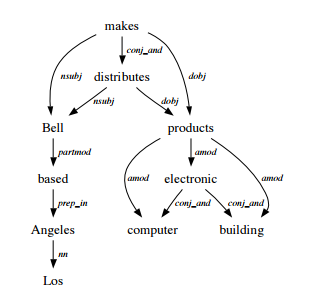
\includegraphics[scale=0.8]{dependency_tree}\end{center}
\caption[Strom vzťahov]{Strom vzťahov}\label{fig:dependency_tree}
\end{figure}

V tomto orientovanom stromovom grafe jednotlivé slová vety predstavujú vrcholy, pričom prechody medzi vrcholmi, hrany, reprezentujú vzťahy medzi nimi.

Ďalšia reprezentácia vzťahov zapisuje vzťahy priamo do vety. Na obrázku \fullref{fig:dependencies_in_sentence} vidíme, že medzi slovami \textit{She} a \textit{looks} je vzťah \textbf{nsubj} - nominal subject, medzi \textit{looks} a \textit{beautiful} je vzťah \textbf{acomp} - adjevtival complement, a v neposlednom rade medzi slovami \textit{very} a \textit{beautiful} je vzťah \textbf{advmod} - adverb modifier~\cite{StanfordDepManual}.
%, ktorý je nominálnou frázou, ktorý je syntaktický subjekt vety. Nadradená časť vo vzťahu nominal subject, tomto prípade \textit{She}, nemusí byť vždy sloveso. Ak je sloveso sponové sloveso, napríklad stať sa, tak koreňom vety je doplnok sponového slovesa, ktoré môže byť prídavné meno alebo podstatné meno.

\begin{figure}[H]
\begin{center}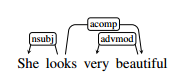
\includegraphics[scale=0.8]{dependencies_in_sentence}\end{center}
\caption[Vzťahy vo vete]{Vzťahy vo vete}\label{fig:dependencies_in_sentence}
\end{figure}

%
% Nástroje na spracovanie prirodzeného jazyka
%
\ifthenelse {\boolean{bachelor}}
{
	%\subsection{Subsection}
	\subsection{Nástroje na spracovanie prirodzeného jazyka}
}
{
	%\section{Subsection}
	\section{Nástroje na spracovanie prirodzeného jazyka}
}
\label{subsec:nlp_nastroje}
V súčastnosti je vyvinutých alebo sú vo vývoji viacero nástrojov, ktoré sa dajú použiť pri spracovávaní prirodzeného jazyka. Vývoj takýchto nástrojov je podporovaný na známych univerzitách ako sú napríklad Princeton, Stanford alebo Camridge, ale samozrejme svoje slovo tu má aj velikán Google. Pozrieme sa bližšie na niektoré z týchto nástrojov, čo ponúkajú a ako sa dajú využiť.

%
% WordNet
%
\ifthenelse {\boolean{bachelor}}
{
	%\subsection{Subsection}
	\subsubsection{WordNet}
}
{
	%\section{Subsection}
	\subsection{WordNet}
}
\label{subsubsec:wordnet}
WordNet je databáza anglických slov vyvíjaná na Princetonskej univerzite. Databáza obsahuje podstatné mena, prídavné mená, slovesá a príslovky, ktoré sú zatriedené do synonymických sád, synsetov~\cite{WordNetPage}.

Slová do synetov sú zaraďované podľa významu. To znamená, že slová auto a automobil, ktoré sú pre svoj význam zameniteľné vo vete, sa zaradujú do rovnakého synsetu. WordNet v súčastnosti (r. 2015) obsahuje 117 000 synsetov. Každý z týchto sysnsetov taktiež obsahuje krátku ukážku použitia slova~\cite{WordNetPage}.

Vo WordNet-e sa nachádzajú aj vzťahy medzi slovami v zmysle nadradenosti. Tým sa myslí, že stolička je nábytok a nábytok je fyzická vec a takto to pokračuje až po najvyššie slovo, od ktorého ,,dedia'' všetky - entita (viď. obrázok \fullref{fig:wordnet_relations}. Okrem vzťahu nadradenosti WordNet obsahuje aj vzťah zloženia. Stolička sa skladá z operadla a nôh. Toto zloženie je typické len konkrétne slovo a neprenáša sa hore stromom nadradenosti,   lebo pre stoličku je typické, že sa skladá z operadla a nôh, ale to už nie je typické pre nábytok.
Prídavné mená obsahujú aj vzťah antonymity, takže slovo \textit{suchý} bude prepojené so slovom \textit{mokrý} ako so svojím antonymom~\cite{WordNetPage}.

Tento nástroj je dostupný vo webovej verzií (viď. obrázok \fullref{fig:wordnet_search}), ale ponúka aj stiahnutie jeho databázových súborov, ktoré sa po splnení licenčných požiadaviek dajú využívať v projektoch.

\begin{figure}[H]
\begin{center}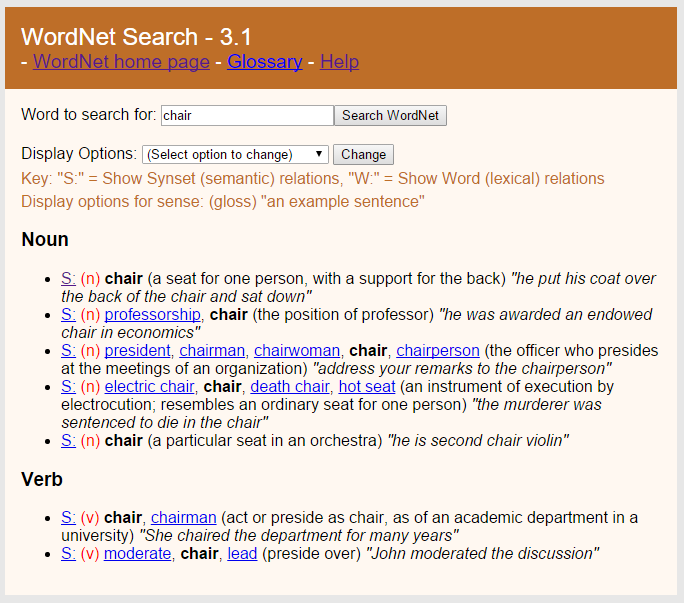
\includegraphics[scale=0.48]{wordnet_search}\end{center}
\caption[Webové rozhranie]{Webové rozhranie}\label{fig:wordnet_search}
\end{figure}

\begin{figure}[H]
\begin{center}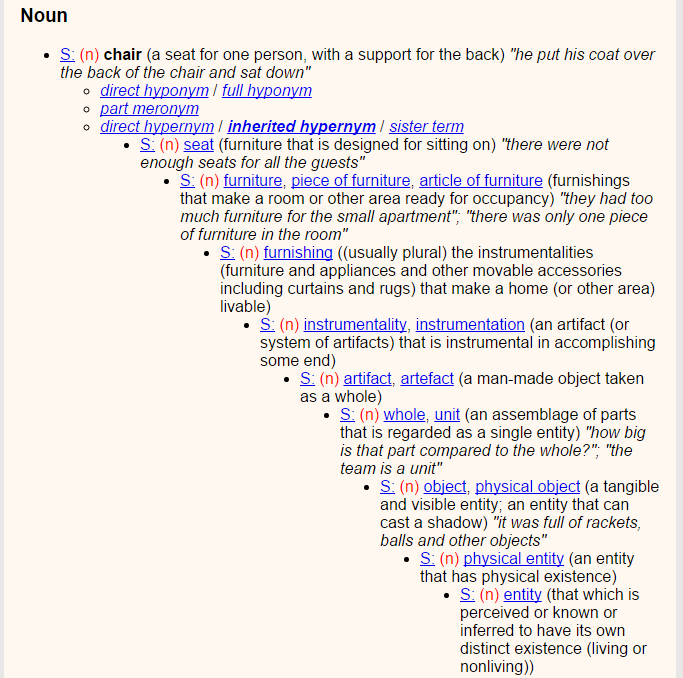
\includegraphics[scale=0.48]{wordnet_search_relations}\end{center}
\caption[Nadradenosť slov]{Nadradenosť slov}\label{fig:wordnet_relations}
\end{figure}

%
% StanfordNLP
%
\ifthenelse {\boolean{bachelor}}
{
	%\subsection{Subsection}
	\subsubsection{StanfordNLP}
}
{
	%\section{Subsection}
	\subsection{StanfordNLP}
}
\label{subsubsec:stanfordnlp}
Nástroj StanfordNLP je vyvíjaný na Stanfordskej univerzite. Skladá sa z niekoľkých softvérov, ktoré sa zameriavajú na úlohy spracovania prirodzeného jazyka popísané v sekcií \fullref{subsec:nlp}. Sú to softvéry \textit{Stanford Parser}, \textit{Stanford POS Tagger}, \textit{Stanford EnglishTokenizer}, \textit{Stanford Relation Extractor} a mnoho ďalších. \textit{Stanford CoreNLP} zahŕňa viacero z týchto softvérov, a práve tento nástroj budeme používať pri spracovaní učebných textov.

Nástroje StanfordNLP sú implementované v Jave, ale sú dostupné aj v iných programovacích jazykoch ako C\#, PHP alebo Python.

Dostupne je aj online webové demo. Na obrázku \fullref{fig:stanfordnlp_online_demo} vidíme výstupy z nástrojov ponúkaných balíkom StanfordNLP pre jednoduchý vstupný text skladajúci sa z jednej vety ,,Martin Nemček is a student at Slovak University of Technology in Bratislava.''.

\begin{figure}[H]
\begin{center}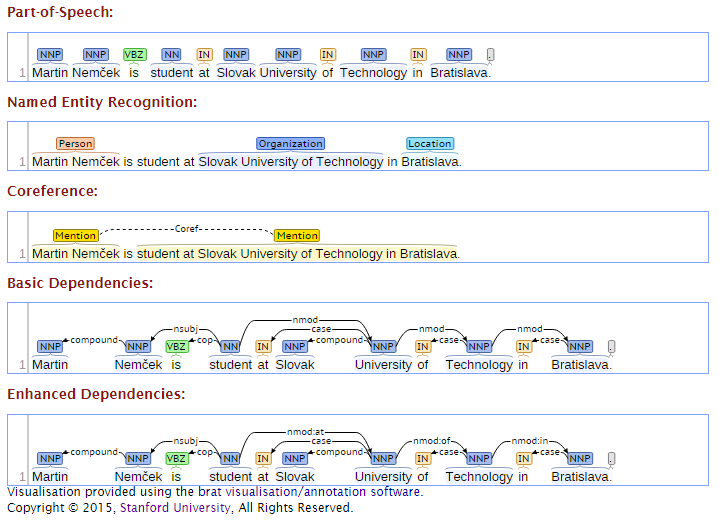
\includegraphics[scale=0.48]{stanfordnlp_online}\end{center}
\caption[StanfordNLP online demo]{StanfordNLP online demo}\label{fig:stanfordnlp_online_demo}
\end{figure}

%
% CambridgeAPI
%
\ifthenelse {\boolean{bachelor}}
{
	%\subsection{Subsection}
	\subsubsection{CambridgeAPI}
}
{
	%\section{Subsection}
	\subsection{CambridgeAPI}
}
\label{subsubsec:cambridgeapi}
CambridgeAPI je vytvorený na Cambridge univerzite. Umožňuje prístup k viacerým rôznym slovníkom. Momentálne tento nástroj ponúka prístup k pätnástim prekladovým slovníkom ako napríklad anglicko-čínsky, anglicko-ruský, anglicko-arabský, anglicko-japonský a ďalšie. Všetky prekladové slovníky majú primárny jazyk angličtinu. Slovenčinu v súčastnosti nepodporuje.

Spomínaný nástroj funguje na princípe dopytovania pomocou HTTP protokolu. Na obdržanie korektnej odpovede je potrebné mať osobný API kľúč. Ten sa dá získať kontaktovaním správcov CambridgeAPI.

%
% Google Ngram
%
\ifthenelse {\boolean{bachelor}}
{
	%\subsection{Subsection}
	\subsubsection{Google Ngram}
}
{
	%\section{Subsection}
	\subsection{Google Ngram}
}
\label{subsubsec:googlengram}
Google Ngram je postavený na ďalšom softvéry tohto giganta, Google Books. V knihách,  napísaných od roku 1500 až do súčastnosti, vyhľadáva výskyty n-gramov. Podporuje len niektoré jazyky, ako angličtina, francúzština, ruština, čínština. Na vyhľadávanie v knihách využíva optické rozoznávanie textu, pričom dokáže spracovať aj regulárne výrazy, avšak tie môžu byť použité iba ako náhrada celého slova, ale nie uprostred slova. Slovné spojenie ,,* Einstein'' spracuje, pričom ,,Albert Einste*n'' nie.

N-gram je podľa oxfordského slovníka definovaný ako postupnosť \textit{n} za sebou idúcich slov alebo znakov. \textit{Martin} je n-gram veľkosti jedna, 1-gram alebo unigram. \textit{Martin Nemček} je n-gram veľkosti dva, 2-gram alebo bigram a tak ďalej, pričom \textit{n} môže byť ľubovolné kladné, celé číslo.

Google Ngram Viewer poskytuje vizualizáciu vyhľadaných dát. Je dostupný vo webovom rozhraní. Na obrázku \fullref{fig:googlengram_visualization} vidno vizualizáciu výskytu mien \textit{Albert Einstein,Sherlock Holmes,Frankenstein} v knihách od roku 1800 do roku 2000.

\begin{figure}[H]
\begin{center}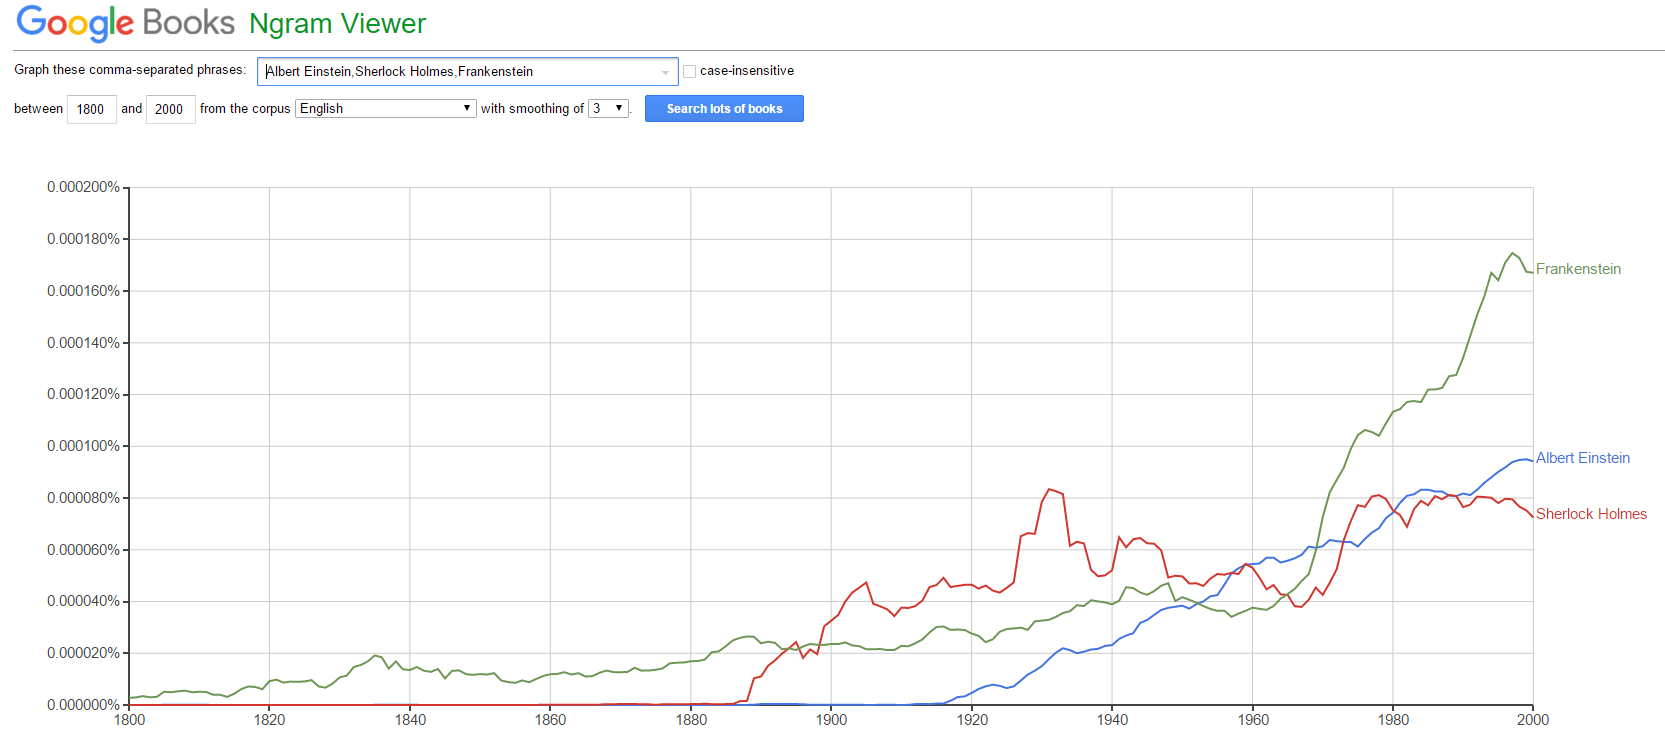
\includegraphics[scale=0.38]{googlengram_visualization}\end{center}
\caption[Google Ngram Viewer]{Google Ngram Viewer}\label{fig:googlengram_visualization}
\end{figure}

Tento nástroj okrem iného ponúka aj surové (angl. raw) dáta na stiahnutie.

%
% AlchemyAPI
%
\ifthenelse {\boolean{bachelor}}
{
	%\subsection{Subsection}
	\subsubsection{AlchemyAPI}
}
{
	%\section{Subsection}
	\subsection{AlchemyAPI}
}
\label{subsubsec:alchemyapi}
AlchemiAPI obsahuje dvanásť funkcií, z ktorých sú niektoré zamerané na úlohy spracovania prirodzeného jazyka popísané v sekcií \fullref{subsec:nlp}, ako napríklad extrakcia entít, extrakcia kľúčových slov, extrakcia vzťahov, ale aj iné zaujímave funkcie, napríklad extrakcia autora z textu.

Na používanie tohto nástroja je potrebné sa zaregistrovať pre obdržanie API kľúču. S týmto kľúčom je tisíc dopytov denne zdarma. Dostupnosť v programovacích jazykoch je široká, kedže ponúka knižnicu v deviatich najpoužívanejších programovacích jazykoch.

Pre AlchemyAPI je dostupné aj online webové demo, viď obrázok \fullref{fig:alchemyapi_visualization}, kde je vidno širokú ponuku, ktorú tento nástroj ponúka.

\begin{figure}[H]
\begin{center}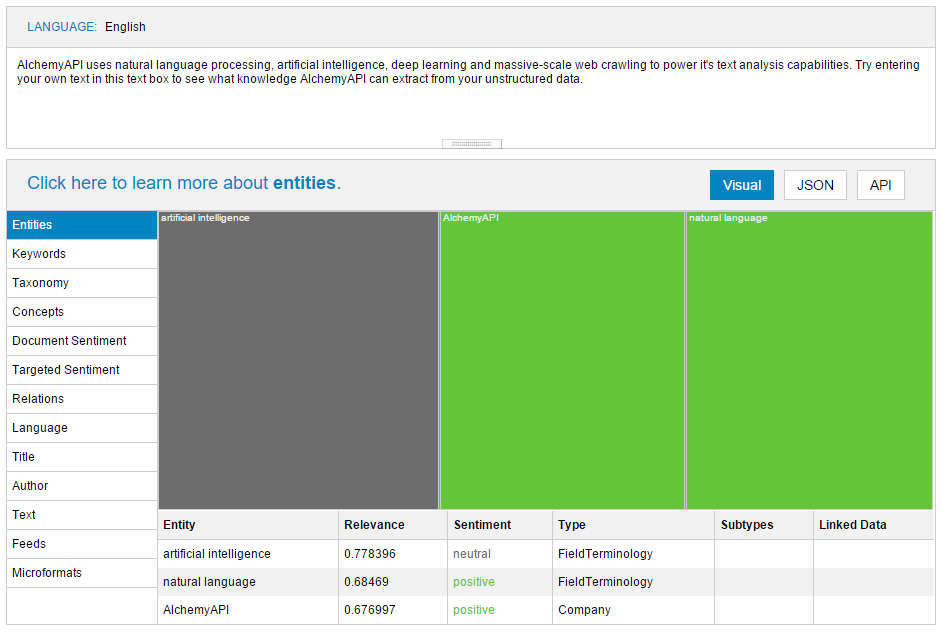
\includegraphics[scale=0.48]{alchemyapi_visualization}\end{center}
\caption[AlchemyAPI online demo]{AlchemyAPI online demo}\label{fig:alchemyapi_visualization}
\end{figure}

Dáta sú vo formáte JSON a okrem spracovania prirodzeného jazyka AlchemyAPI ponúka aj nástroje na extrahovanie obsahu z obrázku alebo rozpoznávanie tvári na obrázkoch.

%
% Smerovanie práce
%
\ifthenelse {\boolean{bachelor}}
{
	%\section{Analysis}
	\section{Smerovanie práce} 
}
{
	%\chapter{Analysis}
	\chapter{Smerovanie práce}
}
V letnom semestri plánujem dokončiť prototyp. To znamená, spraviť používateľské rozhranie, ktoré bude umožňovať vložiť text na spracovanie, zobrazí poznámky a tak isto umožní používateľovi pre ľubovolnú vetu pozmeniť tvar poznámky poznámky. Tieto zmeny sa uložia do databázy a zohľadnia pri ďalšom použití.

Okrem dokončenia prototypu plánujem napísať všetky potrebné kapitoly a dokončiť tým celú prácu.

%
% Opis prototypu
%
\ifthenelse {\boolean{bachelor}}
{
	%\section{Analysis}
	\section{Opis prototypu} 
}
{
	%\chapter{Analysis}
	\chapter{Opis prototypu}
}
V zimnom semestri som implementoval prototyp aplikácie na spoznámkovanie učebného textu.

%
% Notenizer
%
\ifthenelse {\boolean{bachelor}}
{
	%\section{Analysis}
	\subsection{Notenizer} 
}
{
	%\chapter{Analysis}
	\section{Notenizer}
}
\label{subsection:notenizer}
\textbf{Notenizer} je prototyp aplikácie na extrahovanie relevantných informácií z učebných textov. Využíva nástroj Stanford CoreNLP, ktorý je implementovaný v Jave, ale cez IKVM je portnutý aj na C\#. Na ukážke \fullref{code:spustenie_stanford_corenlp} je ukázané prepojenie nástroja StanfordCoreNLP s aplikáciou Notenizer. 
\\

\begin{lstlisting}[ language = csharp, caption={Spustenie StanfordCoreNLP}, label = {code:spustenie_stanford_corenlp}]
String jarRoot = @"stanford-corenlp-3.5.2-models";

Properties properties = new Properties();
// Zvolime, ktore nastroje chceme pouzit.
// pos = part-of-speech tagger
// ssplit = sentence split
// atd.
properties.setProperty("annotators", "tokenize, ssplit, pos, parse");
properties.setProperty("sutime.binders", "0");
properties.setProperty("ner.useSUTime", "false");

// Nastavenie aktualneho priecinku, aby StanfordCoreNLP vedel najst
// vsetky potrebne subory
String currentDirectory = Environment.CurrentDirectory;
Directory.SetCurrentDirectory(jarRoot);
StanfordCoreNLP pipeline = new StanfordCoreNLP(properties);
Directory.SetCurrentDirectory(currentDirectory);

// Vytvorenie anotacie z textu
Annotation annotation = new Annotation(text);

// Spustenie
pipeline.annotate(annotation);
\end{lstlisting}

Údaje získane z tohto nástroja, napríklad POS značky, vzťahy medzi slovami, pozície slov a mnoho ďalších, Notenizer ďalej spracováva. Najdôležitejšie vlastnosti, ktoré sa využívajú v najväčšej miere pri spracovávaní sú závislosti (angl. dependency) medzi slovami vo vete.  

Spracovávaný text sa postupne spracováva po vetách. Každá veta sa samostatne ,,rozparsuje'', spoznámkuje. Vety sa parsujú na základe pravidiel. Na začiatku je daná statická sada pravidiel na spracovanie viet a textov. Po tom, ako sa celý text spracuje, tak sa použité pravidlá uložia do databázy aj s informáciami o pôvodnej vete a novo vytvorenej, zjednodušenej vete. Následne pri opätovnom používaní aplikácie, keď sa začne spracovávať text, tak sa vyhľadajú pre každú vetu pravidlá v databáze, vyberú sa tie s najväčšou zhodou a podľa toho sa spracuje daná veta. Statické pravidla na spracovanie vety sa v tomto prípade použijú len v prípade, ak v sa v databáze nenašli žiadne pravidlá na spracovanie vety, ktoré by pre danú vetu vyhovovali, to znamená, že takúto alebo podobnú vetu zatiaľ Notenizer nespracovával.

Na obrázku~\fullref{fig:example_output} je ukázaný ukážkový výstup prototypu pre vstupný text z wikipédie:
\textit{Czech Republic (Czech: Česká republika) is a country in Central Europe, sometimes also known as Czechia (Czech: Česko). The capital and the biggest city is Prague. The currency is the Czech Crown (koruna česká - CZK). 1€ is about 27 CZK. The president of the Czech Republic is Miloš Zeman. The Czech Republic's population is about 10.5 million. The local language is Czech language. The Czech language is a Slavic language. It is related to languages like Slovak and Polish. In 1993 the Czech Ministry of Foreign Affairs announced that the name Czechia be used for the country outside of formal official documents. This has not caught on in English usage. Czech Republic has no sea; its neighbour countries are Germany, Austria, Slovakia, and Poland.}
\\

Výstup je v tvare [pôvodná veta] ===>> [poznámka z pôvodnej vety].

\begin{figure}[H]
\begin{center}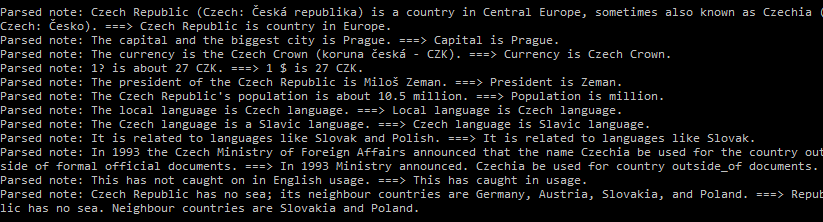
\includegraphics[scale=0.7]{example_output}\end{center}
\caption[Ukážkový výstup prototypu]{Ukážkový výstup prototypu}\label{fig:example_output}
\end{figure}

%
% Pravidlá
%
\ifthenelse {\boolean{bachelor}}
{
	%\subsection{Subsection}
	\subsubsection{Pravidlá}
}
{
	%\section{Subsection}
	\subsection{Pravidlá}
}
\label{subsubsec:notenizer_pravidla}
Pri spracovaní pôvodnej vety sa na túto vetu aplikuje \textit{pravidlo na spracovanie}. Toto pravidlo obsahuje okrem iného zoznam závislostí slov vo vete. Podľa týchto závislostí slov vo vete sa v spracovávanej vete vyhľadajú slová, ktoré majú byť použité v poznámke. Vyhľadávajú sa, okrem iného, podľa POS značiek a indexov vo vete.

%
% Ukladanie a hodnoty pravidiel
%
\ifthenelse {\boolean{bachelor}}
{
	%\subsection{Subsection}
	\subsubsection{Ukladanie a hodnoty pravidiel}
}
{
	%\section{Subsection}
	\subsection{Ukladanie a hodnoty pravidiel}
}
\label{subsubsec:notenizer_ukldanie_a_hodnoty_pravidiel}
Po spracovávaní sa do databázy uložia použité pravidla aj s ostatnými informáciami o pôvodnej a novej vete. Ukladá sa 
\begin{itemize}
	\item Hodnota pôvodnej a novej vety
	\item Zoznam indexov slov, za ktorými bola v poznámke ukončená veta (ak pôvodná veta je súvetie, tak z nej môže vzniknúť viacero poznámok)
	\item Všetky závislostí slov v pôvodnej vete
	\item Všetky závislosti slov v poznámke
\end{itemize}
pričom každá závislosť slov vo vete sa skladá z 
\begin{itemize}
	\item Názvu závislosti
	\item Hodnota governora závislosti
	\item Hodnota dependenta závislosti
	\item Pozícia závislosti vo vete
	\item POS značka a index slova pre governora aj dependenta
\end{itemize}

%
% Vyhľadanie pravidla
%
\ifthenelse {\boolean{bachelor}}
{
	%\subsection{Subsection}
	\subsubsection{Vyhľadanie pravidla}
}
{
	%\section{Subsection}
	\subsection{Vyhľadanie pravidla}
}
\label{subsubsec:notenizer_vyhladanie_pravidla}
Pri spracovávaní vety sa v prvom kroku pozrie do databázy a vyhľadá sa pravidlo na spracovanie tejto vety. Pravidlo sa v databáze vyhľadáva podľa nasledovných podmienok.
\begin{enumerate}
	\item Počet závislostí vety
	\item Názvy závislostí vety
\end{enumerate}
Veta v databáze, ktorej pravidlo chceme použiť, musí spĺňať tieto dve pravidlá. Musí mať rovnaký počet závislostí vo vete ako aktuálne spracovávaná veta a taktiež názvy všetkých závislostí musia sedieť.

Avšak pri týchto podmienkach môže nastať situácia, kedy pre aktuálne spracovávanú vetu bude vyhovovať viacero viet z databázy. V tomto prípade určujeme pravidlo vety s najväčšou zhodou a to sa následne aplikuje.
\\

Zistenie najväčšej zhody ma viacero krokov. Najskôr sa spočítavajú zhody POS značiek governerov a dependentov a indexy slov nezávisle od seba, čiže sa len zisťuje, či spracovávaná veta obsahuje závislosť s nejakou hodnotou indexu, alebo governora, atď.
V druhom kroku sa spočítavajú zhody POS značiek a zároveň aj indexov slov vo vete. To znamená, že sa zisťuje, či sa v spracovávanej vete nachádza napríklad závislosť, ktorej governor ma hodnotu \textit{car} a zároveň má index hodnotu 3.
V poslednom, treťom, kroku sa zisťuje, či sa závislosti zhodujú na všetkých hodnotách, čiže governor a jeho hodnota a index a dependent a jeho hodnota a index \textit{súčasne}.

Tieto tri hodnoty sa na záver spočítajú a tým získame percentuálne ohodnotenie zhody viet.
